\section{Method}
To compare the two learning algorithms, we have written a multi-agent simulation in Python in which agents have to move an object to a certain goal area. In this section, the various components of the simulation will be explained.
\subsection{The Environment}
Figure \ref{2} shows the visual representation of the environment. The environment consists of a 8 by 8 grid in which the agents can move around. There are a number of different types of cells:
\paragraph{Free cells}
These are cells that agents can freely move to. Once an agent or a block moves to a free cell, this cell becomes occupied. They are denoted by dots in the visual representation of the simulation.
\paragraph{Walls}
To make the environment more complex walls were added inside the grid. These cells are occupied, so an agent can never move to them. They are initialized at the start of the simulation and will not change during the simulation. They are represented by hash tags in the visualization.
\paragraph{Block}
The block is an item that has to be transported to a certain goal area by the agents. It occupies one cell, and agents cannot move through it. It can only be moved if it is grasped by all of the agents present in the simulation, and if those agents try to move in the same direction. If the block reaches the goal, an epoch ends. In the simulation, it is denoted by a B.
\paragraph{Goal}
The goal cell is basically the same as a free cell, with the exception that if the block reaches the goal a reward is given to the agents and the run of the simulation ends. Agents can freely move on and over the goal, just like with free cells. In our simulation runs the goal cell was on coordinate (6,6), which is one place left and above from the bottom right corner.
\paragraph{Agent}
The agents occupy one cell, so they cannot move through each other. In the simulation they are represented by A's. The next section describes the agent in more detail. 

\begin{wrapfigure}[20]{r}{.35\textwidth}
\begin{center}
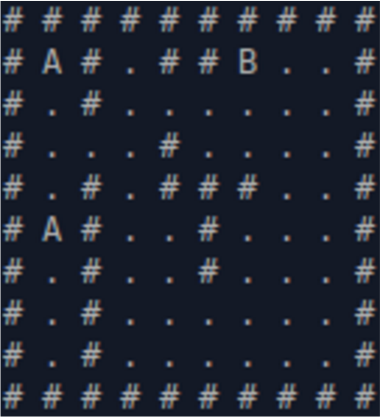
\includegraphics[width=.35\textwidth]{images/environment.png}
\caption{The initial state of the simulation. The \textit{A}'s are agents, while the \textit{B} is the block. The goal is located at coordinates (6,6), which is one place left and above from the bottom right corner.}
\label{2}
\end{center}
\end{wrapfigure}

\subsection{The Agents}
For our simulation, we run the simulation with two agents. At the start of a run, the agents are spawned at their respective start locations which are defined in the algorithm. Each step, an agent can perform one of five actions: \textit{Stay}, \textit{Left}, \textit{Right}, \textit{Up}, \textit{Down} or \textit{Grab}. The actions mostly speak for themselves. An agent can stay where it is, move in one of four directions or grasp the block. The \textit{grasp} action can be performed at any step, but will only do something when an agent is next to the block. Once an agent has grasped the block it will not let go. The move actions \textit{left, up, right} and \textit{down} only do something when the cell the agent wants to move to is actually free. So, for an action to be performed successfully, the algorithm has to check the following things: do the agents move into a space that is occupied? Have the agents grasped the block? And if they have grasped the block, are they moving in the same direction? 

Each step, an agent chooses the best action based on probabilities calculated using its Q-table. Then, the agents perform their actions and update the Q-values. This process repeats itself until the block has reached the goal. After that, a new run starts and the agents are reset to their starting positions. There are two ways for an agent to get a reward: they can either grasp the block to get a reward of 10, or they can push the block onto the goal for a reward of 100. These rewards are used to calculate the Q-values, which is discussed in the following section.

\subsection{The Learning Algorithms}
For this study, we compared two machine learning algorithms: Q-learning and team Q-learning. Both are reinforcement learning algorithms, and they are based on the same principles. The goal of both algorithms is to make sure that the agents find the optimal policy that will result in the highest reward. It can be found through a value iteration method.

\textit{Q-learning} was first introduced by Watkins in 1989 \cite{watkins1989}. It is a model free reinforcement learning technique for multi-agent systems. In our simulation, the agents begin with a Q-table filled with zeros. Each step, they choose one of the six actions with certain probabilities, which are based on the different Q-values. The probabilities are calculated as using a Boltzmann distribution: 
\begin{equation}
	P(a_{k})=\frac{e^{Q(s,a_{k})/ \tau}}{\sum_{l=1}^{m}e^{Q(s,a_{l})/ \tau}}
\end{equation}
Here $s$ is the current state, $m$ is the total number of Q-values for the current state, $a_{k}$ is the $k^{th}$ action and $\tau$ is a parameter that gradually decreases during the simulation. After an action is chosen and a new state $s'$ is reached, the value in $Q(a_{k})$ is updated as follows: 

\begin{equation}
	Q(s,a_{k}) = (1- \varepsilon) Q(s,a_{k})+ \varepsilon (r_k + \gamma \max_{a'} Q[s', a'])
\end{equation}
where $\varepsilon$ is the learning rate between 0 and 1, $\gamma$ is the discount factor (which makes sure that further away states contribute less) and $r_t$ is a reward. From this formula, it becomes apparent that in order to calculate the Q-value for a certain action in a certain state, both the outcome of that action and the outcome of the best possible action in the next state are considered. After each epoch, to make sure the algorithm converges, we update $\tau$: 
\begin{equation}
	\tau_{i} = \tau_{i}-(\tau_{1}-0.1/N)
\end{equation}
where $\tau_{i}$ is the value of the $\tau$-value in epoch i and $N$ is the total number of epochs.

After the agents have reached the goal with the block, their Q-tables are transferred to the next run. This should result in the fact that the agents learn to choose the path that gains them the highest reward. One notable thing in our simulation is that the agents have two separate Q-tables: one for when the agents have grasped the block, and one for when they have not. This is necessary because the best actions change when the agents start moving the block. Thus, they have to optimize two separate paths.

\textit{Team Q-learning} is based on the same principles as Q-learning, and is actually an extension of the Nash Q-learning algorithm \cite{hu}. The primary difference between the two algorithms is that in team Q-learning, the agents share a single Q-table, and the Q-values are based on their joint actions. In this case, each step the best action pair is chosen based on the current position of both of the agents. So, after both agents have taken an action, the Q-value for the joint position and joint action of the agents is still updated with the same formula, but in this case,  $Q(s,a_{k})$ is the Q-value for the shared action $a_{k}$ in the combined state $s$. The probability that a certain action is taken is calculated in a way that is very similar to Q-learning. The main difference is that the probabilities for shared actions are calculated, instead of probabilities for the actions of the individual agents. So, in team Q-learning the agents share a Q-table and action probabilities. With this algorithm, it is like the agents try to cooperate with each other.
